\documentclass[french]{article}
\usepackage[utf8]{inputenc}
\usepackage[T1]{fontenc}
\usepackage{csquotes}
\usepackage[a4paper, total={6in, 8in}]{geometry}
\usepackage{babel}
\usepackage{tocloft}
\usepackage[backend=bibtex]{biblatex}
\usepackage{graphicx}

\addbibresource{biblio.bib}

\cftsetindents{section}{0em}{2em}
\cftsetindents{subsection}{0em}{2em}

\renewcommand\cfttoctitlefont{\hfill\Large\bfseries}
\renewcommand\cftaftertoctitle{\hfill\mbox{}}
\begin{document}

\begin{titlepage}
\newcommand{\HRule}{\rule{\linewidth}{0.5mm}}
\center
\textsc{\LARGE
Université de bordeaux
} \\[1cm]

\HRule \\[0.2cm]
{ \huge \bfseries Analyse des besoins \\[0.15cm] }
{ \bfseries IA pour un jeu de Capture the Flag temps réel en Python\\[0.15cm] }
\HRule \\[1.5cm]
Robin Navarro, Adrien Boitelle, Yann Blanchet\\Alexis Perignon, Alexis Flazinska
\\[1cm]
\today \\ [3cm]
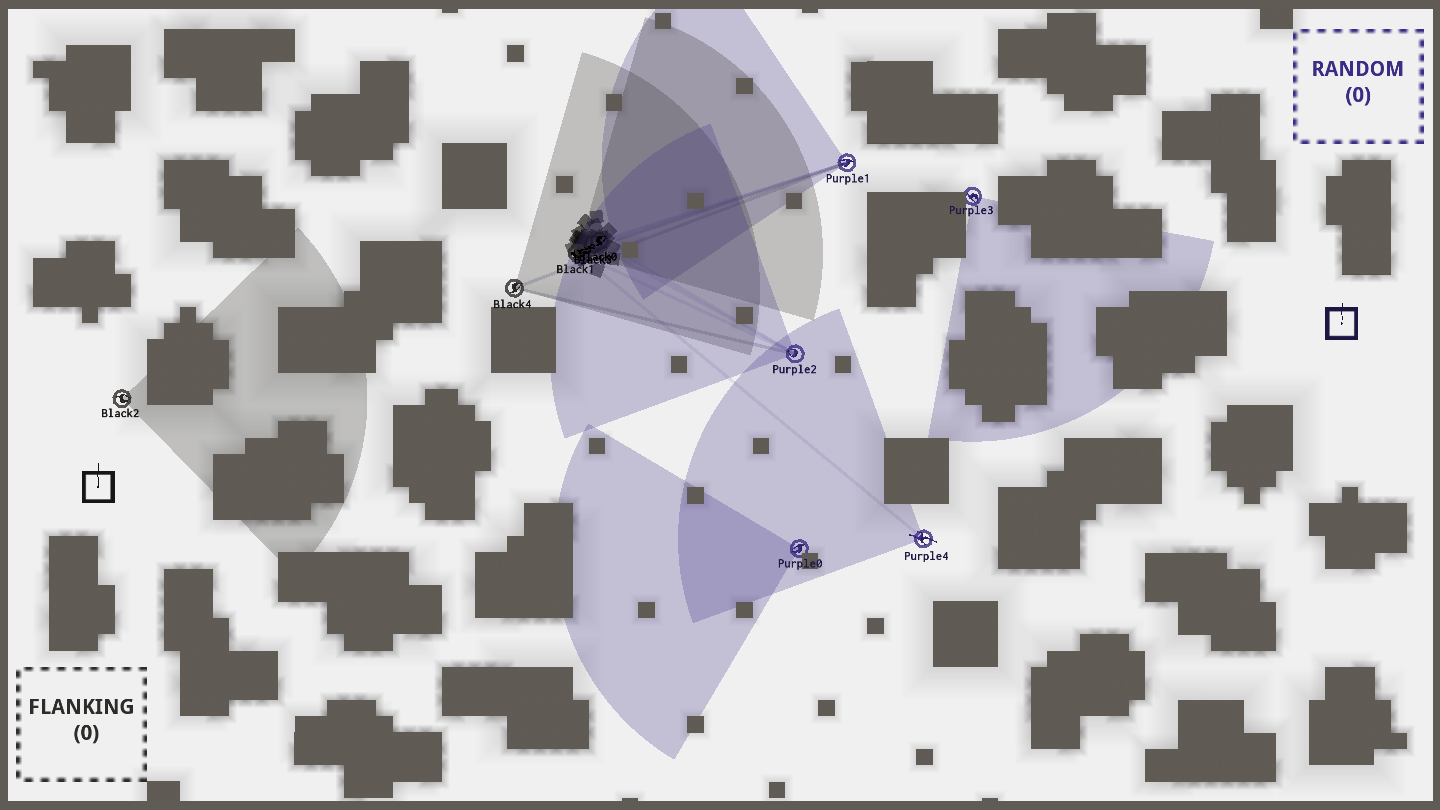
\includegraphics[scale=0.3]{data/illustration.png}{\\openai challenge}
\end{titlepage}


\newpage
\Large
\tableofcontents


\normalsize
\newpage
\section{Description du projet}

Ce projet a pour but la réalisation d'un framework pour un jeu de capture de drapeaux, et la réalisation d'IA pour y jouer.
Le jeu est un capture the flag à deux équipes, ayant chacune le même nombre de bots.
\newline

Chaque équipe évolue sur une carte dont elle a connaissance dès le départ. Tous les bots d'une même équipe commencent dans une zone commune, la zone de départ, et ont pour objectif d'y ramener le drapeau de couleur adverse, tout en gardant leur propre drapeau.
\newline

Chaque bot dispose d'un champ de vision, qui lui permet de détecter des éléments positionnés dans la carte (en particulier les bots adverses). Le champ de vision des bots d'une même équipe est partagé, c'est-à-dire qu'un bot peut voir tout ce que les autres bots de son équipe voient. Les bots peuvent attaquer les membres de l'équipe adverse afin de ralentir leur progression. Si un bot meurt avec le drapeau, il le pose à terre.
\newline

Les IA devront piloter ces bots en temps réel, sur une carte en 2D, en implémentant des stratégies d'équipe.


\section{Analyse de l'existant}
    
Il y a un existant codé en Java pour le moteur de jeu, mais la manière dont il est implémenté ne convient pas au client. En effet, ce moteur repose sur un modèle vectoriel, dans lequel il est plus compliqué d'ajouter des fonctionnalités et de modifier la physique du jeu. C'est pourquoi le client a recommencé l'écriture du moteur en python, en se basant cette fois sur un fonctionnement par "tuile". Mais ce nouveau moteur n'est pas terminé à ce jour. \newline 

La plupart des projets similaires sont des ajouts à deux jeux déjà existant. Par exemple, nous avons trouvé une IA de DeepMind\cite{Jaderberg859} pour le jeu capture the flag, qui se repose sur le jeu Quake. Nous ne pouvons utiliser un jeu existant, car le framework doit pouvoir être facilement réutilisable par des étudiants pour un possible projet dans le cadre de leurs cours. \newline

Suite à nos recherches, nous avons découvert l'existence d'un challenge en ligne datant de 2012 nommé iasandbox.com. Le but de ce challenge était de réaliser une Intelligence Artificielle distribuée pour un moteur de jeu déjà fourni et relié par un serveur. \\Les participants devaient respecter une interface, et implémenter un ou plusieurs bots afin de les faire collaborer et affronter d'autres challengers. Malheureusement, ce site n'est plus accessible suite à un abandon. Nous avons pu trouver des archives web du site, mais le moteur de jeu n'était plus accessible au téléchargement. \\


\newpage
\section{Description des termes techniques}

\begin{itemize}
    \item Framework: Traduit littéralement, signifie "cadre de travail". Désigne un ensemble cohérent de composants éprouvés et réutilisables (bibliothèques, classes, helpers…) ainsi qu'un ensemble de préconisations pour la conception et le développement d'applications.
    \newline
    \item IA: Intelligence artificielle, consiste à mettre en œuvre un certain nombre de techniques visant à permettre aux machines ou programmes d'imiter une forme d'intelligence réelle.
    \newline
    \item Bot: Un programme autonome, qui peut interagir avec des systèmes ou utilisateurs. Très souvent, on parle d'un programme qui se comporte comme un humain dans les jeux vidéos.
    \newline    
    \item Alpha beta: Algorithme de recherche qui sert à réduire le nombre de noeuds calculés par l'algorithme Minimax dans les jeux. L'algorithme Minimax cherche à trouver la meilleure valeur possible d'un plateau de jeu tout en minimisant la meilleure valeur possible d'un plateau de jeu adverse.\newline


    \item Moteur de jeu: collection de code sous forme de bibliothèques et de frameworks afin de réaliser un jeu.
    \newline
    \item Librairie/Bibliothèque/API: un ensemble de fonctions utilitaires, regroupées et mises à disposition afin de pouvoir être utilisées sans avoir à les réécrire.
    \newline
    \item Behavior Tree: Arbre (structure de données) permettant de contrôler le comportement d'une intelligence artificielle, chaque noeud représente une tâche, décision en réponse aux données fournies, ou une structure de contrôle. Permet de réaliser des comportements très complexes et cela en parcourant depuis la racine de l'arbre tout en suivant les branches adéquates en évaluant différentes conditions jusqu'à la décision finale à adopter.
    \newline
    \item Pathfinding: désigne la recherche de chemin entre deux points , noeuds...
    \newline
    \item A*(A star): Algorithme de pathfinding réputé et peu coûteux permettant de rechercher un chemin entre une position initiale et une position finale. Les solutions trouvées par A* sont optimales.
    \newline
    
    \item Frame: Une image affichée à l'écran.\newline 
    
    % Changer pour "l'état du jeu" à la places des images ?
    \item FPS(Frames per second): Fréquence en hertz à laquelle l'état du jeu est calculé.
    \newline
    \item Pygame: Bibliothèque libre multiplateforme qui permet de faciliter le développement de jeux vidéos en langage de programmation Python.
    \newline
    \item Heuristique: Une heuristique est un raisonnement formalisé de résolution de problèmes (représentable par une computation connue) dont on tient pour plausible mais non pour certain qu’il conduira à la détermination d’une solution satisfaisante du problème.
    \newline
    \item Complexité: Évaluation du temps, ressources, et stockage nécessaires à la réalisation d'un algorithme.
    

\end{itemize}{}


\section{Description des besoins}

\subsection{Besoins fonctionnels}
\subsubsection{Besoins utilisateur}
    \begin{itemize}
        \item Fournir une API pour que les IA communiquent avec le moteur de jeu. \\
                Priorité : Essentiel.\\
                L'API doit communiquer aux IA la position de chacun de leurs bots, ainsi que la direction dans laquelle ils regardent. Elle doit aussi communiquer les évènements du jeu, c'est à dire notifier une IA lorsqu'un de ses bots voit quelque chose (ennemi, drapeau, ...), prévenir quand un bot se fait tirer dessus.\\
                En retour, l'IA doit communiquer la destination voulue pour chacun de ses bots, leur vitesse, et des évènements tels que le déclenchement du tir d'un de ses bots.\\
                

        \item Afficher une carte en deux dimensions. \\
            Priorité : Essentiel.
            \begin{itemize}
                \item Afficher les blocs de la carte. Il y a deux blocs de base. Les murs, qui sont solides et bloquent la vue des bots, et des murs transparents. Ils bloquent les bots, mais pas leur champ de vision.
                \item Afficher les zones de chaque équipe.
                \item Afficher les objets dynamiques (bots, drapeau, ...). Les bots sont des cercles.
                \item Afficher le champ de vision des bots. C'est un cône ayant pour base chaque bot, avec une taille variable. \\
            \end{itemize}
            
        \item Fournir un mode de jeu sans affichage graphique. \\
            Priorité : Conditionnel.\\
            Seul les évènements principaux du jeux doivent être affichés (capture de drapeau, mort d'un bot, victoire d'un équipe, ...).\\
            Cet affichage doit pouvoir servir dans le cadre de l'entraînement d'une intelligence artificielle ou pour l'évaluation automatique de projet étudiant.\\

            
        \item Proposer une interface pour qu'un humain puisse jouer contre une IA. \\
            Priorité : Conditionnel \\
            L'interface doit permettre au joueur de sélectionner plusieurs bots, bouger les bots vers une position sélectionnée en cliquant. \\
            Pour faciliter le jeux, les bots doivent tirer automatiquement sur les adversaires qu'ils rencontrent. \\
            Pour tester une interface humaine, dans un premier temps nous vérifierons que dès qu'un bot détecte un bot ennemi dans son champ de vision celui-ci attaque bien automatiquement: un scénario simple serait de mettre un bot contrôlé par l'interface humaine dans le champ de vision d'un autre bot, et bien vérifier qu'il y a attaque.\\
            Il faudra aussi tester le déplacement des bots en cliquant à des positions aléatoires et en vérifiant que les bots ont bien reçu l'ordre de déplacement. \\ 

    \end{itemize}

\subsubsection{Besoins système}
    
    \begin{itemize}
        
        \item Implémenter les règles du jeu. \\
                Priorité : Essentiel.\\
                Les IA doivent avoir à leur disposition 5 bots, se trouvant dans leur zone de spawn respective. Un drapeau se trouve près de chaque base. Un IA qui amène les deux drapeaux dans sa base gagne la partie.\\
                Une contrainte de temps sera définie pour éviter que les IA restent inactives. Si aucune n'a réussi à ramener un drapeau dans sa propre base, alors il y a égalité.\\
                
        \item Charger une carte en mémoire depuis un fichier texte. \\
                Priorité : Conditionnel.
                \begin{itemize}
                    \item Différentes tailles de carte possibles.
                    \item La carte doit être rectangulaire.
                    \item La carte ne doit pas permettre l'évasion des bots de la zone de jeu.
                    \item Le format doit permettre de préciser les zones de chaque équipe et les zones des drapeaux.
                \end{itemize}
                Au moins une carte par défaut doit être disponible. \\
                
        \item Générer des cartes aléatoires.\\
            Priorité : Conditionnel.\\
            Le moteur doit pouvoir générer des cartes correctes (correspondant aux besoins ci-dessus) de manière aléatoire. Les cartes doivent être jouables, c'est-à-dire qu'elles doivent permettre le déplacement des bots depuis leur zone d'apparition jusqu'à la zone du drapeau.\\
            En guise de test, il faudra vérifier que la carte est de la dimension demandée et qu'il est possible de se déplacer des zones de spawn jusqu'aux drapeaux en utilisant A*.\\

        \item Implémenter des IA utilisant l'API du jeu. \\
            Priorité : Essentiel.
            \begin{itemize}
                \item Implémenter une première version basique permettant de montrer le fonctionnement du moteur de jeu. Elle doit effectuer des actions basiques, c'est à dire diriger ses 5 bots vers le drapeau,
                tirer sur les adversaires visibles, capturer le drapeau et le ramener à la base.
                \item Ce comportement simple doit se reposer sur un behavior tree\cite{colledanchise2017behavior}.
                \item Les bots doivent pouvoir réaliser des actions communes, attaquer ensemble, défendre celui qui a le drapeau, défendre le drapeau ... \\
            \end{itemize}
            Pour tester cette IA basique, il faut la faire jouer dans une carte avec des ennemis placés aléatoirement, qui sont immobiles. L'IA doit gagner la partie.\\
            Il faut ensuite tester l'IA sur une carte avec des ennemis placés aléatoirement sur la carte, mais cette fois avec la possibilité de tirer dès qu'un bot se trouve dans son champ de vision. L'IA doit gagner. \\
            Un test un peu plus élaboré consiste à faire jouer l'IA contre une équipe de bots faisant des "rondes" sur la carte, et tirant à vue. Encore une fois l'IA doit gagner pour passer le test.\\
            
            Pour tester la capacité de l'IA à se défendre, on réutilise le test précédent mais en donnant le drapeau de l'équipe à un des bots effectuant des rondes. L'IA doit le récupérer et gagner pour réussir le test.\\
            Une contrainte de temps doit être incorporée dans les tests pour pouvoir mesurer l'évolution des performances de l'IA. \\


        \item Gérer les collisions. \\
                Priorité : Essentiel.
                \begin{itemize}
                    \item Entre les bots et les éléments de la carte.
                    \item Entre les projectiles des bots et les objets du jeu.\\
                \end{itemize}
                Les bots ne doivent pas pouvoir avancer dans une zone considérée comme solide (par exemple un mur). Un moyen pour tester est de lancer une partie avec les bots répartis sur la carte de manière homogène, et en faisant bouger les bots dans des directions aléatoires. Si un bot se retrouve sur une case étant pourtant considérée comme solide, le test échoue.\\
                
                
        \item Détecter les objets dans le champ de vision des bots. \\
            Priorité : Essentiel.
            \begin{itemize}
                \item Transmettre les informations sur les objets vus par les bots aux IA qui les gèrent.
                \item Prendre en compte la transparence des objets de la carte. Par exemple, un bot ne peut pas en voir un autre à travers un mur opaque.\\
            \end{itemize}
            Pour tester le champ de vision des bots, il faut tout d'abord vérifier qu'en mettant un bot sur une carte de jeu, il ne détecte pas les objets n'étant pas dans son champ de vision. Si le moteur détecte une collision, il y a une erreur. \\
            
            Ensuite, il faut tester que le moteur détecte bien la présence d'objet dans le champ de vision d'un bot.
            On place un objet aléatoirement un bot dans le champ de vision du bot. Le moteur doit le détecter, sinon il y a erreur. \\
            Ensuite, il faut placer le bot devant un obstacle opaque, avec derrière un autre bot. Les bots ne doivent pas se détecter entre eux.\\
                
        % Fait partie de l'api non ? Utiliser un angle à la place ?
        \item Déplacer les bots à l'aide d'un vecteur et d'une vitesse.\\
                Priorité : Essentiel.\\
                Le moteur doit pouvoir calculer la nouvelle position des bots à l'aide de deux informations : un vecteur et une vitesse. \\
                
                
        \item Proposer des files de calcul aux joueurs pour les traitements.\\
            Priorité: Conditionnel.\\
            Le moteur doit mettre à disposition des joueurs un mécanisme permettant de réaliser des calculs trop coûteux pour être effectués sur un tour de jeu. Un soin particulier doit être appliqué à la gestion de la priorité des calculs. \\ % Reste à préciser. 

            
        \item Permettre aux bots de pouvoir tirer. \\
            Priorité : Essentiel.
            \begin{itemize}
                \item Respecter une cadence de tir.
                \item Détecter lorsque qu'un bot est touché.
                \item Dire au bot qu'il s'est fait toucher.
                \item Gérer les collision entre le projectile et les éléments de la zone de jeu (par exemple les murs).\\
            \end{itemize}

        \newpage
        \item Gérer la santé des bots.\\
            Priorité : Conditionnel
            \begin{itemize}
                \item Permettre aux bots d'encaisser des dégâts dans la limite de ses points de vie.
                \item Faire réapparaître les bots lorsque leur santé tombe à zéro.
                \item Faire apparaître une représentation visuelle indiquant le nombre de point de vie restant des bots.\\
            \end{itemize}
        

        \item Permettre au bot de récupérer le drapeau. \\
            Priorité : Essentiel.
            \begin{itemize}
                \item Donner au bot le drapeau.
                \item Lâcher le drapeau en cas de mort du bot.
                \item Lâcher automatiquement le drapeau quand le bot revient dans la zone de son équipe.\\
            \end{itemize}
            Pour tester, il suffit de téléporter un bot sur le drapeau. Si le moteur donne le drapeau au bot, le test passe. Sinon, il échoue.\\
        
        \item Permettre au bot de récupérer des items spéciaux \\
            Priorité : Optionnel.
            \begin{itemize}
                \item Différentes armes.
                \item Des bonus tels que: vitesse, gains de vie , téléportation. \\
            \end{itemize}
            Le test est le même que pour le besoin précédent. Il faut téléporter un bot sur les différents objets, et vérifier que le moteur donne bien l'objet au bot. Sinon le test échoue.\\
            
        \item Permettre d'ajouter différents types de bots \\
            Priorité : Optionnel. \\
            Par exemple, permettre l'ajout d'un bot ayant la capacité de détruire certains murs.\\
        
        \item Modification interactive de la carte \\
            Priorité: Optionnel.
             \begin{itemize}
                \item Casser les murs.
                \item Différents types de murs \\
            \end{itemize}
    \end{itemize}


\subsection{Besoins non fonctionnels}
\subsubsection{Besoins utilisateur}
    \begin{itemize}
        \item L'api doit être bien documentée car possiblement destinée à des étudiants.\\
            Quantificateur : Doit être compréhensible par un étudiant qui découvre le projet. \\

        \item L'affichage doit être fluide.\\
            Quantificateur : Le jeu doit pouvoir tourner à 30fps, en utilisant la bibliothèque pygame.\\

        \item Le projet doit être codé en utilisant python. \\
            Quantificateur : Doit être utilisable dans un cours où les étudiants travaillent avec python.\\ %

    \end{itemize}
\subsubsection{Besoins système}
    \begin{itemize}
        \item Le moteur de jeu doit être robuste. \\
            Contrainte, difficulté technique : Le moteur doit continuer à tourner avec des entrées erronées. \\
            Risques et parades : En cas de problème de robustesse, si le moteur est utilisé pour une évaluation automatique, les résultats seront faussés. Il faut donc une gestion des erreurs efficace.\\
            Un moyen pour tester la robustesse du moteur est l'envoi de réponses aléatoires et n'ayant aucun sens au moteur.\\
            Le moteur doit alors continuer à tourner correctement.\\

        \item Les IA doivent répondre rapidement.\\
            Quantificateur : Les réponses doivent être apportées à chaque frame.\\
            Contrainte, difficulté technique : Le code étant en python, il est compliqué d'avoir des performances élevées.\\
            Risques et parades : Le risque est que l'IA ne réponde pas à temps. Dans ce cas, l'IA se fait disqualifier ou doit passer son tour.\\
            \begin{itemize}
                \item Améliorer l'algorithme de pathfinding.
            \end{itemize}
        
        \item Le moteur de jeu doit être capable de traiter efficacement les réponses des IA.\\
            Contrainte, difficulté technique :  La mise à jour de l'état du jeu selon les réponses doit permettre un affichage à 30 fps.\\
            Risques et parades : L'affichage peut perdre de sa fluidité.\\
            Pour tester, on peut donner au moteur des réponses aléatoires mais correctes. Le test doit durer longtemps pour vérifier que le moteur tient dans la durée, sans perte de performances.\\
        
    \end{itemize}

\subsection{Justifications}

Pour l'algorithme de pathfinding, nous avons choisi A* car c'est un algorithme performant et très utilisé dans l'industrie du jeu vidéo, il possède une bonne complexité, $\mathcal{O}(n + m\ log(n))$, $n$ étant le nombre de sommets et $m$ le nombre d'arêtes du graphe représentant le terrain de jeu. De plus, on peut changer l'heuristique pour que les bots puissent s'adapter aux différentes situations (éviter des zones de danger, aller au plus vite vers le drapeau, etc.). \newline

Une première version des bots doit utiliser les behavior trees, car c'est un moyen rapide de prendre des décisions. En effet, avec de nombreux bots sur le terrain et une contrainte de temps sévère, les bots n'ont pas le temps d'utiliser des algorithmes d'exploration d'arbre, tels que l'élagage alpha bêta, de manière efficace. Un autre avantage est de garder un contrôle strict sur le comportement de l'IA et donc de respecter au mieux les stratégies définies à l'avance.\\

Nous avons choisi d'élaborer nous même le moteur de jeu, d'une part en raison de la faible présence d'existant comme expliqué en introduction, d'autre part pour contrôler son évolution, l'ajout de nouvelles fonctionnalités et la maintenance de celui-ci.
\newline

\section{Calendrier prévisionnel}

\centerline{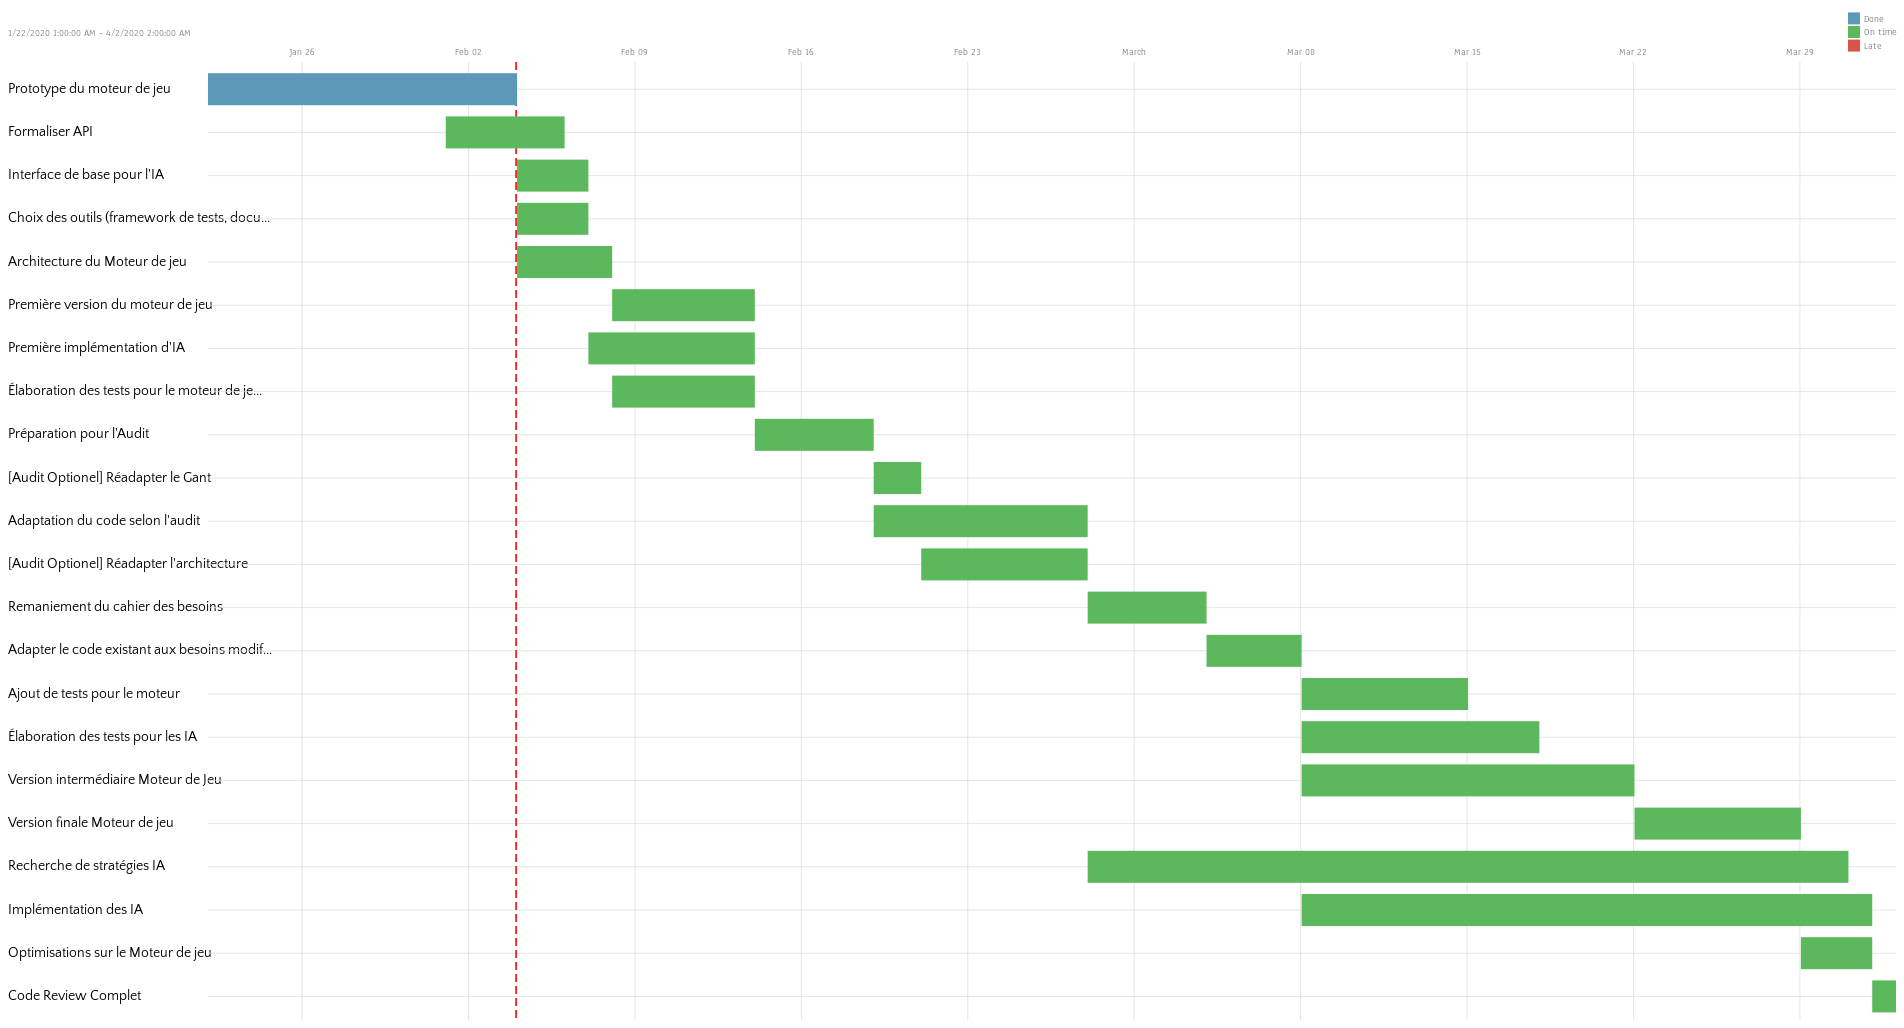
\includegraphics[scale=0.3]{data/gantt.png}}


\section{Bibliographie}

\printbibliography[heading=none]
\nocite{*}
\end{document}